%TODO one idea per paragraph
\chapter{Data and methods}
\label{ch:data_methods}
	In this chapter we describe our approach to answer the scientific questions stated during the introduction. The first section of this chapter introduces the datasets used during this study and the underlying causes for using them. For each dataset, we shortly describe by which approach it is derived and what are the fundamental meta-data properties. Additionally, if possible we try to give for each dataset an accuracy assessment, ideally provided by other research groups if available. Finally, we describe our idea behind using the data and how we acquired and filtered it. The second and last section of this chapter is focused on the applied methodology to prepare our analysis and results. For each processing step we give a short description of the methodical background and describe the core functionality of our processing algorithms. For implementing our processing algorithms and visualizing our results we selected individually the programming language or software which fulfills best the requirements. These approaches are encapsulated in a reusable software design to easily reproduce, alter or reuse our algorithms and findings.

\section{Data}
\label{sec:data}
%TODO first paragraph/sentence "SO WHAT" why we used the dataset
	\begin{table}[ht]
		\centering
		\caption[Datasets used in this study]{\textbf{Datasets used in this study}}
		\label{tab:datasets}
		\begin{tabular}{lll}
			\hline
			Data & Type & Source \\\hline
			Global Forest Change & spatial & \citet{Hansen2013}\\
			GlobeLand30 & spatial & \citet{Chen2015}\\
			Intact Forest Landscape & spatial & \citet{Potapov2017}\\
			Aboveground Woody Biomass & spatial & \citet{Baccini2015}\\
			Global Soil Organic Carbon Content & spatial & \citet{FAO2018}\\
			Global Administrative Areas & spatial & \citet{Hijmans2018}\\
			Soil Organic Carbon Change & empirical & \citet{Don2010}\\
			\multirow{3}{*}{Ecosystem Service Values} & \multirow{3}{*}{empirical} & \citet{Groot2012}\\
			&& \citet{Costanza2014}\\
			&& \citet{Siikamaki2015}\\\hline
		\end{tabular}
	\end{table}
	The table \ref{tab:datasets} shows a comprehensive overview of the applied datasets for this study. Spatial datasets comprises vector as well raster data, while empirical data is extracted from the cited publications. The subsequent sections describe each dataset in further detail.

	\subsection{Global Forest Change}
		\ac{GFC} 2000-2012 Version 1.0 is the first high-resolution dataset that provides a comprehensive view of the annual global forest cover change between 2000 and 2012 \citep{Hansen2013,Li2017}. The initial \ac{GFC} dataset released by \citeauthor{Hansen2013} has been extended by recent releases, which encompass the annual forest cover changes between 2000-2013, 2000-2014, 2000-2015 and 2000-2016, respectively. All versions of this dataset have in common, that they are derived from growing season imagery captured by the remote sensing satellite Landsat 7 \ac{ETM+} enhanced by band metrics of other sensors like Quickbird imagery, existing percent tree cover layers from Landsat data, and global \ac{MODIS} percent tree cover \citep{Hansen2013}. On the satellite imagery, a time-series spectral metrics analysis is applied to gather the global forest extent at 2000 as well as the annual forest loss and the accumulated gain for the period 2001 till 2012. Hence, \ac{GFC} comprises three independent data layers tree cover, annually forest loss and forest gain divided into 10x10 degree tiles by the geodetic coordinate system \ac{WGS84} (EPSG:4326) with a spatial resolution of 1 arc-second per pixel (approximately 900 Km$^2$ or 30x30 m). Furthermore, across the provided \ac{GTiff} layers the pixel data is coded in unsigned 8-bit integers. Hansen et al. defined trees as all vegetation taller than 5 meters for their study. For each pixel covered by trees, a canopy density ranging from 0 t0 100 \% is computed. Forest loss is defined as a stand displacement disturbance leading from a forest state to a non-forest state (e.g. canopy density >50 \% to 0). Therefore the underlying cause of forest loss ranges from anthropogenic impacts to natural causes. Tree cover gain is defined as the inverse of loss where the canopy density must exceed 50 \% to get recognized.

		\citeauthor{Hansen2013} reports as an accuracy assessment of tree cover loss a producers accuracy of approximately 83 \% for the tropical region. The mapped tree cover gain is probably an underestimation of the true gain with a producers accuracy of 48 \% and a user's accuracy of 81 \%. 

		This dataset is publicly available for download without any constraint. For a convenient bulk download, the dataset homepage provides a "\verb|*.txt|" files comprising the \ac{URL} of the tiles for each sub-dataset. The spatial location of an image can be directly determined from the file name within the \ac{URL}. Each file name has a common pattern shown by the following expression: "\verb|Hansen_VERSION_LAT[NS]_LNG[WE]|". LAT (latitude) and LNG (longitude) refer to the top left corner coordinates of a raster image, whereas these coordinates are only given in natural numbers. The orientation of the image on the hemisphere is determined by the four cardinal directions N (north), S (south), W (west) and E (east). For this project, we require all three sub-datasets, namely: Treecover2000, loss-year, and gain. The data acquisition is automatized with a Python script by using the \ac{stdlib} modules urllib and re. At first, the Python script downloads the provided "\verb|*.txt|" files and creates a list data structure, where each \ac{URL} is an element of this list. After, it cycles through the list and extracts the corner coordinates from the file name by means of a \ac{REGEX}. These corner coordinates and cardinal directions are converted to valid latitude and longitude coordinates between $[-90, 90]$ and $[-180, 180]$, respectively. Now, an image is only downloaded if it is within the study extent between $[-20, 30]$ latitude. The acquired image tiles in total 678 are shown in the top panel (green squares) in figure \ref{fig:dataset_tiles}.
		\begin{figure}[ht]
			\centering
			\includegraphics[scale=.93]{img/tiles}
			\caption[Map of downloaded dataset tiles]{\textbf{Map of downloaded dataset tiles:} This map shows the acquired image tiles for this study. From top to bottom in green Global Forest Change (GFC) dataset tiles (Treecover2000, loss-year and gain), the land cover dataset GlobeLand30 (GL30) image tiles in red, and in blue the Aboveground Biomass (AGB) dataset tiles. The orange filled shapes highlight countries within the tropical zone.}
			\label{fig:dataset_tiles}
		\end{figure}

	\subsection{GlobeLand30}
		\ac{GL30} is the first global land cover dataset with a 30 meter per pixel spatial resolution that provides a comprehensive view on the distribution of 10 different land cover classes (table \ref{tab:gl30_classes}) over the entire globe \citep{Chen2017}. Currently, this dataset is available for two different time periods 2000 and 2010 \citep{Chen2015}. The pixel values of this dataset are coded in unsigned 8-bit integers and as coordinates system, it uses \ac{WGS84} in \ac{UTM} projection. \ac{GL30} can be downloaded as a \ac{GTiff} raster mosaic where each image covers 6x5 degrees \citep{Chen2014}. For detecting the land cover classes \citeauthor{Chen2015} used a so-called \ac{POK} oriented approach and satellite imagery from Landsat \ac{ETM+} \citep{Chen2015}. \citeauthor{Chen2015} divided the mapping process into different stages where each land cover type is detected separately and deleted subsequently from the source satellite image. The applied mapping order is water bodies, wetland, snow and ice, cultivated land and forest, shrubland, grassland and bare land synchronous. To detect the pixels of a selected land cover type the following pixel level classifiers are used: \ac{DT}, \ac{SVM} or \ac{MLC}. After pixel detection, the adjacent pixels are grouped as an aggregated land use object. These objects are subsequently validated by expert knowledge and the gained knowledge is used as a feedback loop to improve the automatized classification.

		\citeauthor{Chen2015} estimates an overall mapping accuracy of 80.33 \% and 78.6 \% for 2000 (only validated in Shaanxi, China) and 2010 (global), respectively \citep{Chen2015}. Several research groups besides \citeauthor{Chen2015} validated the mapping accuracy of \ac{GL30} at different regions and scales. \citeauthor{Arsanjani2016} estimates an overall accuracy of 77.9 \% for Iran and an accuracy >80 \% for Germany \citep{Arsanjani2016a,Arsanjani2016}. Yang et al., Cao et al. and Jacobson et al. estimate the accuracy of 82.4 \%, 80.1 \% and 83.1 \% for China, Nepal, and East Africa, respectively \citep{Yang2017,Cao2016,Jacobson2015}. Unfortunately, no study focused on validating the mapping accuracy for regions exclusively within the tropical zone.

		\citeauthor{Chen2015} donated the \ac{GL30} land cover mapping to the \ac{UN} but it is not accessible for public download. The download is restricted to users who register on the dataset homepage but the registration process is not working properly. Fortunately, the supervisor of this work had already an account otherwise it would be impossible to receive a copy of the dataset. A registered user must fill an order application to get access to the image tiles. The application form must contain the tile identifiers and the selected time period. Tile identifiers have the following common pattern: "\verb|[NS]ZONE_LAT_NAME|" where zone refers to the \ac{UTM} zone between $[1, 60]$, N (north) or S (south) to the cardinal direction, and LAT (latitude) to the latitude coordinate of the top left corner. For better usability the homepage provides an interface for selecting the required image tiles but the selection of multiple tiles did not work. As well a vector file is provided which contains the dataset tile polygons with assigned identifiers. This file was used to select all required tiles within the tropical zone between approximately $[-23, 23]$ degrees (\ac{WGS84}). Figure \ref{fig:dataset_tiles} presents the selected images in red at middle panel. The corresponding image identifiers are converted to a single line string and copied to the application form. After submitting the form the order will be checked and approved within two weeks. After one week we received a two weeks limited access to a password protected \ac{FTP} server where we downloaded 716 raster images. Due to the several restrictions, this process of selecting and downloading could not be automatized with one pipeline. Only the selection and string conversion were automatized with a throwaway script.
		\begin{table}[ht]
			\centering
			\caption[Classification schema of the GlobeLand30 product]{\textbf{Classification schema of the GlobeLand30 product:} The code column is the assigned pixel value, type the corresponding land cover type and definition explains in broad terms which types of surfaces fall into the land cover type \citep{Chen2017}.}
			\label{tab:gl30_classes}
			\begin{tabular}{rlp{10.3cm}}
				\hline
				Code & Type & Definition \\\hline
				10 & Cultivated land & Used for agriculture, horticulture and gardens, including paddy fields, irrigated and dry farmland, vegetable and fruit gardens, etc. \\
				20 & Forest & Covered by trees, vegetation covers over 30\%, including deciduous and coniferous forest, and sparse woodland with cover 10-30\%, etc. \\
				30 & Grassland & Covered by natural grass with cover over 10\%, etc.\\
				40 & Shrubland & Covered by shrubs with cover over 30\%, including deciduous and evergreen shrubs, and desert steppe with cover over 10\%, etc.\\
				50 & Wetland & Covered by wetland plants and water bodies, including inland marsh, lake marsh, river floodplain wetland, forest/shrub wetland, peat bogs, mangrove and salt marsh, etc.\\
				60 & Water bodies & In land area, including river, lake, reservoir, fish pond, etc.\\
				70 & Tundra & Covered by lichen, moss, hardy perennial herb and shrubs in the polar regions, including shrub-, herbaceous-, wet- and barren-tundra, etc.\\
				80 & Artificial surfaces & Modified by anthropogenic influence, including all kinds of habitation, industrial and mining area, transportation facilities, and interior urban green zones and water bodies, etc.\\
				90 & Bareland & With vegetation cover lower 10\%, including desert, sandy fields, Gobi, bare rocks, saline and alkaline land, etc.\\
				100 & Snow and ice & Covered by permanent snow, glacier and icecap\\\hline
			\end{tabular}
	\end{table}

	\subsection{Intact Forest Landscapes}
		An \ac{IFL} is a mosaic of undisturbed forest patches and naturally treeless ecosystems without signs of human activity and large enough to maintain all native biological diversity \citep{Potapov2017}. Due to the fact that \ac{IFL} comprises different intact natural landscape patterns like primary forests, non-forest ecosystems, temporary treeless areas after a natural disturbance, and water bodies the term is not congruent to the term primary forest defined by the \ac{FAO} \citep{FAO2012}. But as mentioned \ac{IFL}s includes large patches of primary forests with a minimum extent of 500 Km$^2$, therefore, primary forests can be extracted from the layer. Still, there are smaller fragments of primary forest outside of the \ac{IFL}s. In regards to the extent an \ac{IFL} has a minimum size of 500 Km$^2$, a minimum width of 10 Km, and a minimum corridor/appendage width of 2 Km. Further an \ac{IFL} should not contain any of the following: ecosystem alternation, fragmentation by infrastructure and disturbance, and areas altered or managed through agriculture, logging, and mining. For mapping and detecting \ac{IFL}s \citeauthor{Potapov2017} used Landsat imagery and several auxiliary data sources like \ac{GFC}, and national transportation maps. The dataset can be downloaded as a \ac{SHP} file with the coordinate reference system \ac{WGS84}. Each polygon in the \ac{SHP} represents an \ac{IFL} patch at a certain location on our planet at the time period 2000.

		Data acquisition is pretty straight forward the \ac{IFL} dataset public accessible for download. As mentioned it is a \ac{SHP} so you must only download a single compressed archive. The download is automatized with a Python script by using the \ac{stdlib} modules urllib and threading \citep{Rossum2018}.

	\subsection{Aboveground Woody Biomass}
		The \ac{AGB} raster dataset is prepared by \ac{GFW} by an adapted approach of \citeauthor{Baccini2012} \citep{Baccini2012,Baccini2015,Baccini2017}. For the year 2000, this dataset estimates the aboveground biomass density per pixel in Mg C ha$^{-1}$ (megagram carbon per hectare), and the confidence per pixel at a spatial resolution of approximately 1 arc-second (approximately 900 Km$^2$ or 30x30 meter). The dataset covering the global tropical zone as a mosaic of \ac{GTiff} raster images where each tile of the mosaic has the \ac{CRS} \ac{WGS84} and is coded in a float. For deriving biomass density \ac{GFW} used canopy metrics from \ac{GLAS} \ac{LIDAR} footprints and several regional and forest-specific allometric equations. The resulting \ac{GLAS} \ac{AGB} estimates are used as labels to train regional specific \ac{RF} models based on Landsat 7 \ac{ETM+} top-of-atmosphere reflectance, tree canopy density of \ac{GFC}, elevation data, and climate data as predictor variables. After these models are subsequently applied to the entire study extent to predict the biomass content for each pixel. Additional an uncertainty layer is prepared accounting for the errors from allometric equations, the \ac{LIDAR} based model, and the random forest model.

		The \ac{AGB} raster mosaic is publicly available on the homepage of \ac{GFW}. As mentioned, the dataset covers only the tropical zone, therefore we acquire the entire mosaic. The \ac{GFW} homepage provides an \ac{GeoJSON} \ac{API} to receive the actual \ac{URL} of each raster image. If a request is sent to this \ac{API} the server responded with a \ac{GeoJSON} feature collection. The collection contains as attributes the \ac{URL}s of the biomass images, the \ac{URL} of the uncertainty layers, and the rectangular bounds of each image. The data acquisition is automatized by means of Python and the \ac{stdlib} modules urllib, threading, and the open source library geopandas \citep{Rossum2018,McKinney2010}. At first, the \ac{GeoJSON} is downloaded via an \ac{API} call and eventually stored on disk. Next, we iterate the features of the \ac{GeoJSON} collection and extract the \ac{URL}s (biomass and uncertainty) of each tile. These \ac{URL}s are downloaded and subsequently stored on disk. During the downloads of the uncertainty layers, the \ac{GFW} server answered repeatedly with a 404 (Not found). Therefore the uncertainty layers are not available. In total we downloaded 105 different image tiles, their extent and spatial location are shown in blue at the bottom panel of figure \ref{fig:dataset_tiles}.

	\subsection{Global Soil Organic Carbon}
	%TODO references for wosis, hwsd, and other data products
		The \ac{GSOCmap} is a joint project between \ac{GSP} and \ac{ITPS} to produce a global \ac{SOC} content map by a country-driven approach. In the year 2018, the first iteration of this map in version 1.0 was released and shortly followed by 1.1 (new country submission by Rwanda) and 1.2 (new country submissions by Chile and Colombia). As the short release cycle suggests the mapping project is intended as a long-lived dataset which will improve over time and by new country submissions. Till now 67 (approximately 63 \% of the global land mass) different countries submitted their country based \ac{SOC} estimates. To foster the national \ac{SOC} mappings the \ac{ISRIC} provides several covariate datasets like national \ac{DEM} maps, annual spectral remote sensing data or national soil type grids. Additionally, the contributors can join a mapping training and use the \ac{GSOCmap} cookbook as guidance for their mapping efforts. As an exchange, each country shares its national \ac{GSOCmap} by compliance of several criteria e.g. reporting of the Meta-data of the \ac{SOC} sampling (sample timeline, sample depth, bulk density etc.), uncertainty assessment, and the applied methods for estimating and interpolation of the \ac{SOC} content. For interpolating the guide organizations suggest the following approaches: simple geo-matching, class-matching, \ac{MLR}, \ac{RF} or \ac{SVM}. The national maps are aggregated to the final \ac{GSOCmap} with a target resolution of 30 arc-seconds (approximately 1 Km$^2$) in the \ac{CRS} \ac{WGS84}. The dataset is one single raster image as \ac{GTiff} coded in float covering the entire globe where each pixel value is the \ac{SOC} content in Mg C ha$^{-1}$ at a soil depth of 0-30 cm \citep{FAO2018}.

		The product is validated by comparing the pixel level estimates with soil sampling data from various soil databases (WoSIS, HWSD, etc.). In total 312122 samples where divided into three sub-levels (<150 Mg C ha$^{-1}$, >150 Mg C ha$^{-1}$, and all samples) and subsequently computed the \ac{ME}. The \ac{ME} of the entire sample space and <150 Mg C ha$^{-1}$ suggests that the mean \ac{SOCC} estimate is an overestimate of 1.6 and 4.5 Mg C ha$^{-1}$ respectively. All samples with a \ac{SOCC} content >150 Mg C ha$^{-1}$ show an underestimate by approximately 165 Mg C ha$^{-1}$ in the mean. Additionally, an uncertainty assessment was prepared to estimate a \ac{SD} between $\pm$ 0-16 t ha$^{-1}$ for the tropical zone. Unfortunately, is this assessment pretty rough and till now not available as a product. The \ac{GSOCmap} in comparison with other global \ac{SOC} products has the lowest \ac{RMSE}. In summary, the prepared validations show evidence that the \ac{GSOCmap} is a conservative data product with a tendency to underestimate the \ac{SOCC}.

		The dataset is publicly available at the homepage of the \ac{FAO}. As mentioned it consists of one raster image, therefore we download it by means of a Python script without any additional steps.

	\subsection{Soil Organic Carbon}
		\citeauthor{Don2010} performed the first study of tropical \ac{SOC} change for soil depth between 0 and 30 cm. For the study, a global meta-analysis is applied by using 358 (153 published an peer-reviewed) different studies to estimate \ac{SOC} change for 12 major \ac{LUC} types. The base date is derived from 39 different tropical countries covering all continents. Unfortunately, Africa and East-Asia are under-sampled whereas South-America has the best data coverage. The meta-analysis is restricted to mineral soils therefore all wet soil types are excluded from the analysis \citeauthor{Don2010}. The 12 \ac{LC} transitions encompass the following \ac{LC} types: primary forest, secondary forest, grassland, cropland, and perennial crops. Primary forest is defined as natural vegetation without human impacts which includes natural grassland and shrubland. Secondary forest is managed forests and regrown forests after partial destruction of the old stand. Grassland comprises pastures for livestock but excludes natural grasslands. Cropland comprises annual crops like maize or beans and perennial crops could be coffee or sugar cane. For our study we used only the \ac{SOC} change estimates for these \ac{LUC} types which correspond to the \ac{GL30} and \ac{IFL} classification schema. The actual values are shown in table \ref{tab:soc_factors}.
		\begin{table}[ht]
			\centering
			\caption[Relative soil organic carbon change for certain land-use change types]{\textbf{Relative soil organic carbon change for certain land-use change types:} The Land-use change columns from and to define the LUC type with the corresponding relative Soil Organic Carbon (SOC) change and the Standard Error of the Mean (SEM) \citep{Don2010}.}
			\label{tab:soc_factors}
			\begin{tabular}{lrr}
				\hline
				LUC type & \multicolumn{2}{c}{Relative SOC change} \\
				From$\rightarrow$To & [\%] & SEM \\\hline
				Primary forest$\rightarrow$Grassland & -12.1 & $\pm$2.3 \\
				Primary forest$\rightarrow$Cropland & -25.2 & $\pm$3.3 \\
				Primary forest$\rightarrow$Secondary forest & -8.6 & $\pm$2.0 \\
				Secondary forest$\rightarrow$Grassland & -6.4 & $\pm$2.5 \\
				Secondary forest$\rightarrow$Cropland & -21.3 & $\pm$4.1 \\\hline
			\end{tabular}
		\end{table}

	\subsection{Ecosystem Service Values}
	%TODO sort table as: co, dg, wb
	%TODO add  2007 Int'I\$ y^-1 ha^-1, Geary-Khamis Dollar
		\note{Pending},
		which type of ecosystem services are included in the biome types
		\begin{table}[ht]
			\centering
			\caption[Selection of Ecosystem Service Values (ESV) used in this study]{\textbf{Selection of Ecosystem Service Values (ESV) per biome used in this study:} ESV per biome and its monetary value in Int.\$ ha$^{-1}$. Dg refers to data from \citeauthor{Groot2012}, Co from \citeauthor{Costanza2014}, and Wb from \citeauthor{Siikamaki2015}.\citep{Groot2012,Costanza2014,Siikamaki2015}}
			\label{tab:esv_factors}
			\begin{tabular}{lrrr}
				\hline
				Biome & Dg & Co & Wb \\\hline
				Cropland & - & 5,567 & -\\
				Forest tropical & 5,264 & 5,382 & 1,312\\
				Grass/Rangelands & 2,871 & 4166 & -\\
				Wetlands & 25,682 & 140,174 & -\\
				Lakes/Rivers & 4,267 & 12,512 & -\\
				Urban & - & 6,661 & -\\\hline
			\end{tabular}
		\end{table}

	\subsection{Auxiliary}
	%TODO cite natural earth
		As auxiliary data for country boundaries and the selection of continental regions we downloaded with Python the \ac{GADM} and Natural Earth layers as \ac{SHP} files \citep{Hijmans2018,Rossum2018}.

\section{Methods}
\label{sec:methods}
%TODO flowchart of all processes
	Figure \note{flowchart and reference} shows an overview of the entire processing pipeline. The following sections describe detailed the applied approach for each step in figure. The order of appearance is from left to right. 

	For implementing our processing algorithms we selected for each task the technology which fulfills best the requirements. Python is our core language for implementing our processing algorithms because it supports a easy implementation of multiprocessing which is heavily used in this project. From the Python \ac{stdlib} we used the following libraries: urllib, re, unittest, time, math, logging, collections, bisect, and enum. Additionally for geo-processing we used the following open source libraries: numpy, pandas, fiona, geopandas, shapely, matplotlib. The entire frontend of our Python source code is aggregated in a Jupyter Notebook and available on GITHUB. This ensures that everyone interested can easily reproduce the findings of our project. JavaScript and the additional modules papaparse and the google maps api are used for programming a small web app for cross validation of land use predictions. R is used for hypothesis testing. Bash is used to aggregate large raster datasets as vrt files. To prepare map visualizations we used QGIS. Dia is used for preparing flowcharts and GIMP is used for image post-processing.

	\subsection{Preprocessing}
	%TODO flowchart add masking 
	%TODO improve image caption
	%TODO add total number of tiles per datasets
		Before we apply further analysis, we have to generalize the used datasets. As introduced in the data section do we use datasets which differ largely in their metadata properties, for example, single-tiled or multi-tiled images, used \ac{CRS}, spatial resolution, and file type. Therefore, our goal should be to develop a process which creates an image stack of equal meta-data for each location in our study extent. In further descriptions, we will refer to this stack as \ac{AISM}. As target \ac{CRS} for our \ac{AISM} we chose \ac{WGS84} and as target extent for the mosaic, we use the bounding box of the \ac{GL30}-2010 tiles. The following paragraph explains how we developed the alignment algorithm by means of Python and the additional open source libraries rasterio, geopandas, and shapely \citep{Rossum2018,McKinney2010}.

		The first exercise of the preprocessing algorithm is to detect all tiles covering the extent of our template tiles. At first, we create for each multi-tiled dataset a polygon mask as \ac{SHP}. This mask contains the spatial extent of each tile within a dataset and as attribute the corresponding file identifier. If the dataset tiles are not in \ac{WGS84} the extracted bounds are subsequently reprojected to this \ac{CRS}. During the masking process, we recognized that the raster mosaic bounds of both \ac{GL30} datasets (2000 and 2010) generate re-projection errors. These errors showed up as polygons spanning the entire globe but one tile can only fill its \ac{UTM} zone extent. Further analysis revealed that all tiles located in \ac{UTM} zone 1 and 60 overflowing the maximum and minimum longitude coordinates of these zones. As solution we excluded all tiles within \ac{UTM} zone 1 and 60 from further processing, namely: n01\_00, s01\_00, s01\_10, s01\_15, s01\_20, s60\_00, s60\_05, s60\_10, s60\_15, and n53\_00. The described steps can be found as well in figure \ref{fig:preprocessing_flowchart}. Now, as the figure suggests we determine the intersection between these mask layers and group the intersecting tiles by our template tile. Next, we create for the template tile a re-projection profile (warp profile) and apply it subsequently to all intersecting tiles based on the following rules: if from one dataset more than one tile intersects merge them followed by re-projection or if only one tile intersects just re-project it. As introduced the \ac{GSOCmap} consist only of one single tile with a spatial resolution of approximately 1 Km$^2$, so it must only re-project and re-sampled by the nearest-neighbor approach. We select from the \ac{IFL} layer all polygons within our template warp profile and convert them to a raster layer where intact forest patches are coded by a one in an 8-bit unsigned integer. The last step of the alignment process is the rounding of the \ac{AISM} bounds to full integer degrees and a subsequent clipping of each tile to this rounded bounds. The entire work-flow is presented in figure \ref{fig:preprocessing_flowchart} and results in a \ac{AISM} shown in figure \ref{fig:aligned_tiles}. Finally, we create a polygon mask of our \ac{AISM} and store for each polygon the corresponding dataset tiles. This mask is used as a file index for the next algorithms.
		\begin{figure}[ht]
			\centering
			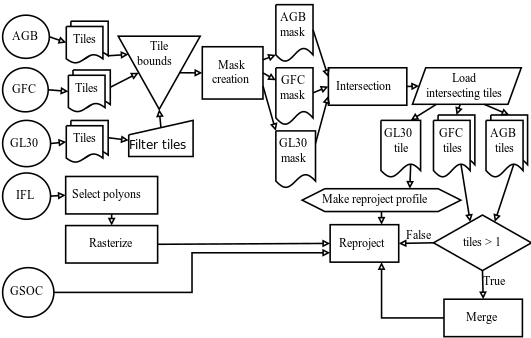
\includegraphics[scale=.9]{img/align}
			\caption[Tile alignment algorithm]{\textbf{Tile alignment algorithm:} For the multi-tiled datasets (multi-document symbols) a mask is created by extracting the tile bounds. Next, the intersection between these masks is determined to identify superimposing data and the corresponding tiles are loaded from disk. \ac{GL30} tiles are used as a template by creating the re-project profile and subsequently applying it to intersecting tiles. From the \ac{IFL} layer only polygons within the re-project area are selected and subsequently converted to a raster layer.}
			\label{fig:preprocessing_flowchart}
		\end{figure}
		\begin{figure}[!ht]
			\centering
			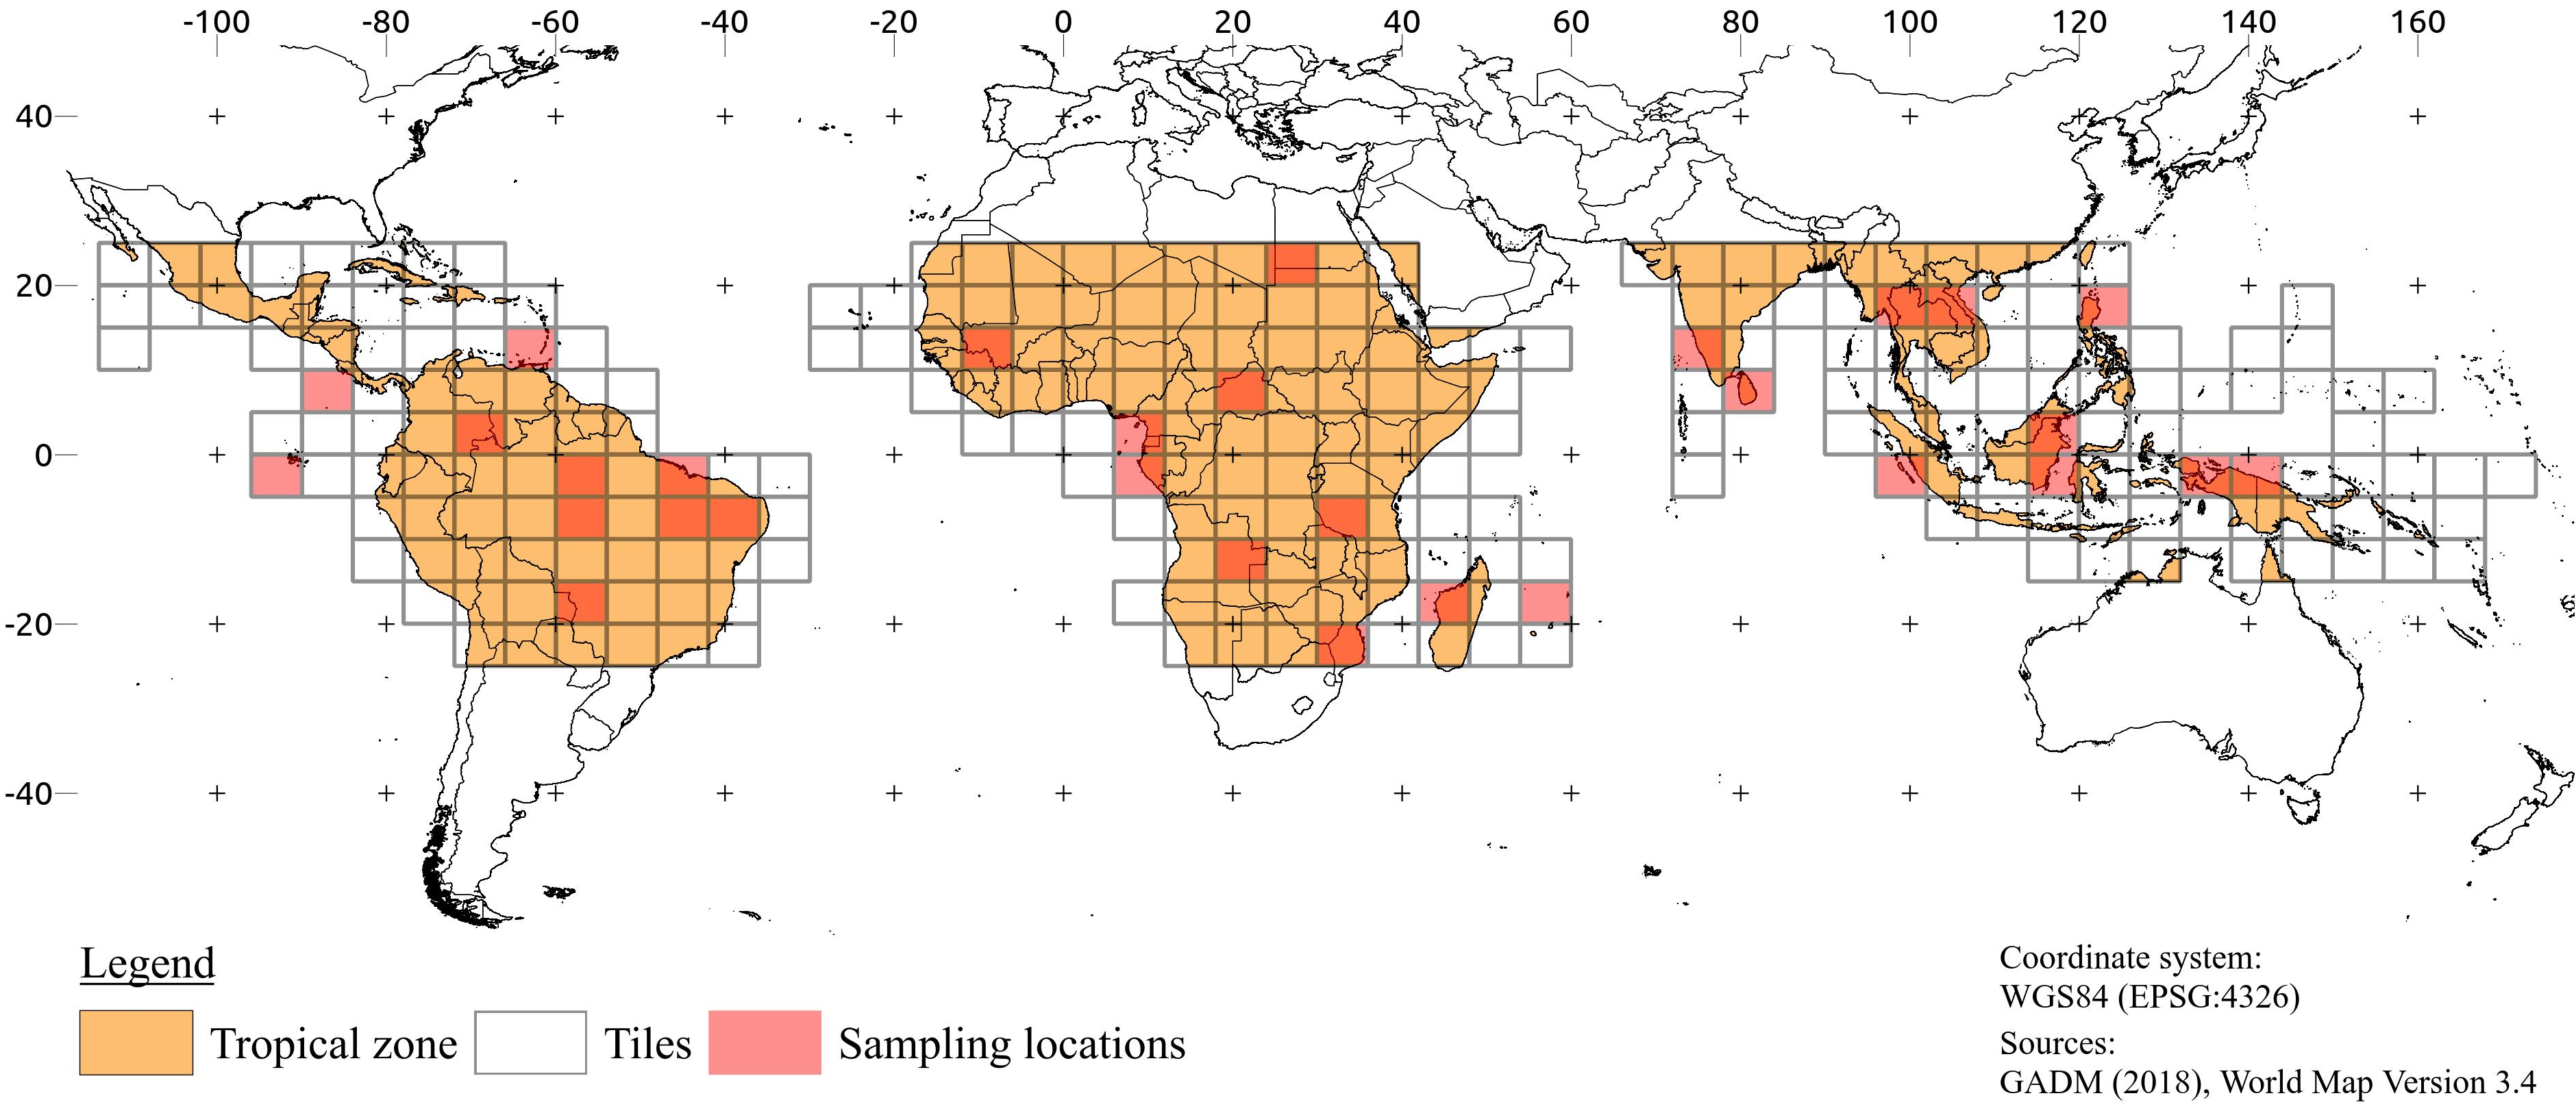
\includegraphics[scale=.95]{img/method_overview_frameless}
			\caption[Aligned raster images and sampling locations]{\textbf{Aligned raster images and sampling locations:} The map shows the location of the aligned multi-image stack tiles as black-framed, square-sized polygons. The sampling locations for accuracy assessment are represented in red, Countries within tropical range appear in orange. Vertical blue lines separate the tiles into the three continental regions Latin America, Africa, and Asia/Australia.}
			\label{fig:aligned_tiles}
		\end{figure}

	\subsection{Deforestation} 
		\subsubsection{Forest definition}
			To determine the proximate drivers of deforestation we combined the information of the two datasets \ac{GFC} and \ac{GL30}. However, both differ in their definition of tree cover by canopy cover threshold as introduced in section \ref{sec:data}. \ac{GFC} detects tree cover over the entire canopy density interval of $(0,100]$, while the \ac{GL30} threshold is set to > 10 \%. To successfully extract stable land cover transformation by superimposing both layers we must first harmonize the tree cover definition of both strata. We hypothesize that if both layers agree on tree cover they should also agree if a transition to a non-forest state occurs. To harmonize both definitions we have the opportunity to vary the canopy density of \ac{GFC} to determine at which density class the similarity between them is at its maximum. Then, we use the examined maximum similarity canopy density to filter the tree cover loss and gain layer.

			To determine the similarity between \ac{GL30} 2000 and \ac{GFC} reference tree cover we used the \ac{JI}. The \ac{JI} or coefficient of community is a simple measure of similarity between two pairs of a binary population or a measure of the degree of spatial overlap between two images \citep{Sampat2009}. This index was first applied by \citeauthor{Jaccard1912} to compare distributions of rare alpine flora in 1912 \citep{Jaccard1912}, and since it is a widely used metric across multiple fields. If we compare two binary images, let $a$ be the magnitude where both images (Img$_1$, Img$_2$) have an agreement represented as a pixel value of one. Let $b$ the magnitude where Img$_1$ is zero and Img$_2$ is one, while $c$ represents the inverse expression. Finally, assume that $d$ is the magnitude of elements where both images are zero. The matrix in table \ref{tab:jaccard_matrix} shows that the computation of this coefficients $a$, $b$, $c$, and $d$ can be expressed as a set of boolean operations. Equation \ref{eq:jaccard_index} shows how the \ac{JI} is computed by substitute integer values for the variables. This computation can be reduced to two boolean operations for a major performance increase. The \ac{JI} is always within the closed interval $[0,1]$, where an index of one or zero means a complete similarity between both populations or a complete disagreement, respectively. The relationship between $a$ and \ac{JI} is near linear \citep{Shi1993}. The first step to compute the \ac{JI} for our raster images is to extract the tree cover from the \ac{GL30} 2000 land cover by setting all pixels with values $\neq$ 20 to zero and values $=$ 20 to one. Next, we extract from the \ac{GFC} reference tree-cover pixel values within the half-opened interval of the following canopy density classes and set them to one: $(0,100]$, $(10,100]$, $(20,100]$, and $(30,100]$. Therefore, we test four different tree cover definitions for \ac{GFC}. The first excludes canopy densities $\leq$ 0\%, the second $\leq$ 10\%, the third $\leq$ 20\%, and the fourth  canopy densities $\leq$ 30\%. We will refer to this \ac{JI} of different canopy density classes as JI$_0$, JI$_1$, JI$_2$, and JI$_3$. For all 269 tiles of our \ac{AISM}, we calculate the \ac{JI} existing between \ac{GL30} and \ac{GFC} for the four above-mentioned forest definitions by using equation \ref{eq:jaccard_index}. The algorithm is implemented in Python by using numpy's ability to perform boolean operations between large matrices. As parameters, the function expects two matrices with the same dimensionality in $R^{n*m}$ and a boolean indicating if the function should return the coefficient matrix as well. The previously described preprocessing steps are implemented as an extra function. This function requires as parameter two raster layers, a list of integer values to consider as \ac{GL30} forest cover (default is 20), and the lower bounds of the canopy density intervals to consider for computation.
			\begin{table}[ht]
				\centering
				\caption[Jaccard Index coefficient matrix]{\textbf{Jaccard Index coefficient matrix:} $a$ is the magnitude of agreement, $d$ is the magnitude of disagreement, $b$ and $c$ are the magnitudes of partial disagreements among both images. The computation of these coefficients can be expressed as boolean operations on matrices.}
				\label{tab:jaccard_matrix}
				\begin{tabular}{lccc}
					\hline
					& & \multicolumn{2}{c}{Img$_1$} \\
					& State & 1 & 0 \\\hline
					\multirow{2}{*}{\STAB{\rotatebox[origin=c]{90}{Img$_2$}}} & 1 & $a=|\mathbf{X_1} \land \mathbf{X_2}|$ & $b=|(\mathbf{X_1} \land \mathbf{X_2}) \oplus \mathbf{X_2}| $ \\ 
					& 0 & $c=|(\mathbf{X_1} \land \mathbf{X_2}) \oplus \mathbf{X_1}|$ & $d=|\neg ( \mathbf{X_1} \lor \mathbf{X_2})|$ \\\hline 
				\end{tabular}
			\end{table}
			\begin{equation}
			\label{eq:jaccard_index}
				JI = \frac{a}{a+b+c} = \frac{|\mathbf{X_1} \land \mathbf{X_2}|}{|\mathbf{X_1} \lor \mathbf{X_2}|}
			\end{equation}

			To optimize the overall tree cover similarity between both datasets we must test which canopy density class yields the highest agreement over our study extent. To test the significance of the difference between two correlated samples, we decided to apply the non-parametric Wilcoxon signed-rank test \citep{Wilcoxon1945}. This test requires paired data from the same population, at least an ordinal scale of measurement, each sample pair is independent, and the dependent variable can be expressed as a continuous probability \citep{Lowry2019}. Further, an advantage of this test is that we don't have to assume a normal distribution for our sample population. Our sample population fulfills these requirements.  The test procedure is implemented in R because this language is mainly intended for this kind of statistical analysis. We exported the computed \ac{JI} from our Python environment and applied a cross-testing in R. In our case, cross testing is defined as the test of all possible \ac{JI} combinations. Further, we applied a two- and one-sided Wilcoxon test because we want to examine if there is a significant difference and which direction has the similarity distribution. To address the higher probability of family-wise error in multiple comparisons we used a Holm correction. Before we applied the examination of the distribution we separated our population into three independent regions, namely Latin America, Asia/Australia, and Africa highlighted by the vertical blue lines in figure \ref{fig:dataset_tiles}. Latin America, Asia/Australia, and Africa comprised 82, 86, and 101 image tiles, respectively. Additionally, we excluded from the analysis all samples where JI$_0$ is zero because this tiles from our \ac{AISM} did not contain any pixels covered by trees. In Latin America, Asia/Australia, and Africa we excluded 6, 13, and 15 tiles. We tested continental differences in tree cover agreement to inspect regional dependencies and global differences. The results from the global testing are used to determine our definition of tree cover. Further, we compared differences of tree cover agreement between the continental regions by applying a Wilcoxon rank-sum test also known as Mann-Whitney U test. We applied a Benjamini and Hochberg correction to the test results.
 
		\subsubsection{Proximate deforestation driver}
		\label{subsubsec:methods_proximate_deforestation_driver}
		%TODO flowchart add reclassification
		%TODO how aggreagted: hexagonal, natural earth for countries (low resolution from R)
		%TODO mention your definition of ppd classes, goes after haversine equation
			Based on our forest definition developed in the previous section we want to classify all the tropical deforestation within a canopy density of $(10,100]$ percent between 2001 till 2010. Additionally, we must consider the mean miss-classification rate of 52 \% by previous findings of \citeauthor{Seydewitz2017} \citep{Seydewitz2017}. Therefore we have to develop a feasible method to resolve this issue.

			For classifying the proximate drivers of deforestation we selected the following raster images from our \ac{AISM}: \ac{GFC} reference tree-cover, \ac{GFC} annual losses, \ac{GFC} gain, and the \ac{GL30} \ac{LC} classification of 2010. Now, we apply to each raster image stack the following described operations. From the reference tree-cover images, we select all pixels where the canopy density is within the half-open interval of $(10,100]$ percent and set them to one (true). The same exercise is applied on the annual losses stratum by setting all forest loss pixels within the time period 2001 till 2010 to one (true). After, both layers are combined with a logical AND operation to select our target deforestation pixels. Finally, we build the Hadamard product (element-wise multiplication) of the target deforestation layer and the \ac{GL30} \ac{LC} stratum to classify the pixels with a deforestation event. For classifying forest regrowth we filtered the \ac{GFC} gain layer to consider only tree-cover gain within our target temporal resolution and target canopy density. After, the filtered stratum is aggregated with our classified deforestations by using the Hadamard product of both layers. We will refer to this proximate deforestation driver layers as PDD. Figure \ref{fig:driver_flowchart} shows an overview of the classification process. The classification algorithm is implemented as a Python function which requires a parameter the previously named raster layers. Additionally the target canopy density and time period is freely selectable for experimental variations. The described filtering and aggregation steps are implements as binary matrix operations for fast processing of large data sizes by means of numpy.
			\begin{figure}[ht]
				\centering
				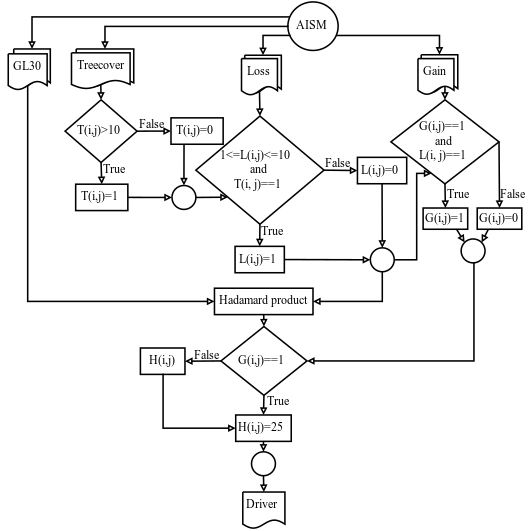
\includegraphics[scale=.68]{img/driver_flowchart}
				\caption[Classification of proximate deforestation drivers]{\textbf{Classification of proximate deforestation drivers:} For the classification of the proximate deforestation drivers the following layers are required GL30 2010, GFC tree cover, annual losses, and gain. From tree cover we select all pixels within the canopy density interval $(10,100)]$. The tree cover mask is used to select the appropriate annual losses within the time interval $[2001,2010]$. To predict a land cover change after a deforestation event we use the Hadamard product.}
				\label{fig:driver_flowchart}
			\end{figure}

			After classifying the proximate deforestation drivers we developed an approach to smooth the misclassified pixels based on an approximated probability. We define misclassifications as sites where the \ac{GFC} annual loss data predicts deforestation but the \ac{GL30} stratum still classifies them as forest. The first step of our reclassification is to cluster the misclassified pixels with the Hoshen-Kopelman algorithm \citep{Hoshen1998}. The clustering algorithm is implemented as a part of the \ac{GDAL} library and can be called through the rasterio interface. For this project, we used the following parameters: connectivity 4 and a boolean mask where only pixel values $=$ 20 are true. Now the algorithm creates for each pixel cluster a polygon. After we created a squared sized buffer with a side length of 500 x 500m around the polygon centroid (the geometric midpoint of the polygon). Because \ac{WGS84} is not an equal area \ac{CRS} we must compute for each tile the buffer size separately. To compute the buffer size in image coordinates we used the Haversine formula in equation \ref{eq:haversine_function} to determine the on-ground resolution in meter on pixel level. Where $d$ is the great-circle distance between two latitude, longitude pairs $\varphi_n, \lambda_n$ and $r$ is the earth radius of approximately 6378137 m. Because this computation is expensive we assumed that the pixel resolution is equal for an entire raster tile. After extracting the buffer we counted the most frequent class under exclusion of pixels with a value of 0, 20 or 255 within the buffer. Finally, if the most frequent class is defined we reassigned this class value to the cluster. The reclassification algorithm is implemented as a Python function which requires as parameters a proximate driver raster image, a list of elements which should be interpreted as occupied cells for the clustering, pixel values which should be excluded from counting, the side length of the buffer, and the on-ground resolution. 
			\begin{equation}
			\label{eq:haversine_function}
				d = 2r\arcsin\left(
				\sqrt{
						\sin^2\left(\frac{\varphi_2-\varphi_1}{2}\right)+\cos\left(\varphi_1\right)\cos\left(\varphi_2\right)\sin^2\left(\frac{\lambda_2-\lambda_1}{2}\right)
				}
				\right)
			\end{equation}

		\subsubsection{Accuracy assessment}
		%TODO convert expressions to i,j
		%TODO findings during accuracy asssement
		    For examining the accuracy of our \ac{PDD} predictions we used a confusion matrix (also known as two-way frequency tables, error matrix or contingency tables). These matrices are commonly used for an accuracy assessment of land cover classifications and enable the computation of marginal and conditional distributions \citep{Congalton1991,Foody2002}. Table \ref{tab:methods_confusion_matrix} shows a general model of a confusion matrix. Foundation for an accuracy assessment by means of a confusion matrix is a collection of ground-truth samples which can be compared with the class predictions for these samples produced by a classification algorithm. For the preparation of our accuracy assessment, we have to extract a collection of pixel samples with a deforestation occurrence from our proximate driver maps (further also called predictions). Next, we compose a set of ground-truth for these predictions (further also called references).
			\begin{table}[ht]
				\centering
				\caption[A general model of a confusion matrix]{\textbf{A general model of a confusion matrix:} $X_1$, ... , $X_n$ denote classification categories of two independent raters. $x_{n,n}$ are the actual samples sorted into the categories where the values in the diagonal show the agreement between both raters. The remaining cell values account for the disagreement between the two raters. $\sum$ column and row show the marginal distribution and N is the total number of samples.}
				\label{tab:methods_confusion_matrix}
				\begin{tabular}{lccccc}
					\hline
					& & \multicolumn{3}{c}{Reference} & \\
					& Cls & $X_1$ & $\cdots$ & $X_n$ & $\sum$ \\\hline
					\multirow{4}{*}{\STAB{\rotatebox[origin=c]{90}{Predict}}}
					& $X_1$ & $x_{1,1}$ & $\cdots$ & $x_{1,n}$ & $x_{1.}=
					\displaystyle\sum_{i=1}^{n} x_{1,i}$ \\ 
					& $\vdots$ & $\vdots$ & $\ddots$ & $\vdots$ & $\vdots$ \\ 
					& $X_n$ & $x_{n,1}$ & $\cdots$ & $x_{n,n}$ & $x_{n.}=\displaystyle\sum_{i=1}^{n}x_{n,i}$ \\\hline 
					& $\sum$ & $x_{.1}=\displaystyle\sum_{i=1}^{n}x_{i,1}$ & $\cdots$ & $x_{.n}=\displaystyle\sum_{i=1}^{n}x_{i,n}$ & $\sum\sum=N$ \\\hline
				\end{tabular}
			\end{table}

			To create our collection of ground-truth data we draw randomly 10 image tiles from all three continental regions (Latin America, Africa, Asia/Australia) namely the following tiles: 25N 024E, 20N 096E, 20N 102E, 20N 120E, 15N 066W, 15N 012W, 15N 072E, 10N 090W, 10N 018E, 10N 078E, 05N 072W, 05N 006E, 05N 114E, 00N 096W, 00N 060W, 00N 048W, 00N 006E, 00N 096E, 00N 114E, 00N 132E, 00N 138E, 05S 048W, 05S 042W, 05S 060W, 05S 030E, 10S 018E, 15S 060W, 15S 042E, 15S 054E and 20S 030E where the first part is the latitude coordinate and the last part is the longitude coordinate of the upper left corner. From each tile, we sampled by random 200 pixels which total to 6000 samples over the entire study region. The sampling is realized with our own raster sampling algorithm build in Python by means of the open source libraries numpy and rasterio. As mentioned in the previous section do we superimpose two datasets and only a certain amount of pixels per tile is classified as a proximate driver. Therefore, the sampling algorithm should only draw samples from occupied/classified pixels without replacement. The algorithm expects as parameters a raster image, the total number of samples to draw, a list of pixel values which should be interpreted as occupied cells, the affine transformation matrix of the raster image, and a seed for the random number generator. If occupied cells are set the algorithm will create a binary mask where each occupied cell is set to one relative to the input raster image. Otherwise, it sets all pixel values greater or less than zero to one. After, the row and column coordinates of each one are extracted from the mask and converted to a flat list of coordinate tuples. Next, it draws the predefined number of samples from the list by a random order and uses the image coordinates to get the pixel value from the raster image. If an affine transformation matrix is provided the image coordinates are converted to real-world coordinates. The seed argument ensures that on every algorithm rerun the samples are drawn. For our sampling we set the parameters to the following values: samples 200, occupied pixels \ac{GL30} class values and 25 for regrowth, the affine matrix of the corresponding raster image, and the seed is 42. The per tile samples are stored as a \ac{CSV} file.

			For the collection of ground-truth data, we used a visual interpretation of satellite and aerial imagery provided by Google Maps. We developed a small JavaScript web application to access the imagery via the Google Maps \ac{API}. The application expects as input a \ac{CSV} file with the sampling coordinates. After upload of a sample file the user can cycle through the entries and the map jumps automatically to the coordinates of the sample. Now a reference label can be assigned to the coordinates by visual interpretation of the imagery. We subsequently assigned to all 6000 samples a reference label and downloaded the results as \ac{CSV}.

			Finally, we developed a Python class to compute the confusion matrix. The constructor of the class requires a list of reference and prediction labels. With the provided arguments it creates the confusion matrix. Further, it computes the following marginal and conditional distributions: overall accuracy $OvAc$ by dividing the sum of classification agreements by the sample total $N$ (equation \ref{eq:overall_accuracy}), the producer accuracy $PAc_{.n}$ by dividing the category agreement by the column category total (equation \ref{eq:producer_accuracy}), the error of commission $Com_{.n}$ (Type II error) by dividing the category disagreement by the column category total (equation \ref{eq:comission_error}), the user accuracy $UAc_{n.}$ by dividing the category agreement by the row category total (equation \ref{eq:user_accuracy}), the error of omission $Om_{.n}$ (Type I error) by dividing the category disagreement by the row category total (equation \ref{eq:omission_error}), and the Cohens Kappa by substituting equation \ref{eq:cohen_coefficient} and \ref{eq:overall_accuracy} into equation \ref{eq:kappa_coefficient}.
			\begin{equation}
			\label{eq:overall_accuracy}
				p_0=OvAc = \frac{\displaystyle\sum_{i=1}^{n}x_{i,i}}{N}
			\end{equation}
			\begin{equation}
			\label{eq:producer_accuracy}
				PAc_{.n} = \frac{x_{i,i}}{x_{.n}}
			\end{equation}
			\begin{equation}
			\label{eq:comission_error}
				Com_{.n} = \frac{FN_i}{x_{.n}}
			\end{equation}
			\begin{equation}
			\label{eq:user_accuracy}
				UAc_{n.} = \frac{x_{i,i}}{x_{n.}}
			\end{equation}
			\begin{equation}
			\label{eq:omission_error}
				Om_{n.} = \frac{FP_i}{x_{n.}}
			\end{equation}
			\begin{equation}
			\label{eq:cohen_coefficient}
				p_c = \frac{1}{N^2}\displaystyle\sum_{i=1}^{n} x_{.i} \cdot x_{i.}
			\end{equation}
			\begin{equation}
			\label{eq:kappa_coefficient}
				Kappa = \frac{p_0-p_c}{1-p_c}
			\end{equation}

	\subsection{Emissions}
	%TODO pdd classes switch to 10, 25, 30, 40, 80, 90
		Land cover change respectively deforestation releases carbon emissions. These emissions can be grouped to different categories like emissions from transportation, biomass removal, changes of soil carbon dynamics, processing of certain kind of commodities etc.. During the previous sections we developed an approach to predict the change of tree cover driven by proximate causes like conversion to cropland or else. Now we can use these predictions to approximate the CO$_2$ emissions uprising from this land cover transitions. For this study, we focus on the emissions emitted by biomass removal and from changes of soil carbon stock. The first paragraph is focused on the estimation of emissions from biomass removal and the second section tries to approximate the impact of land cover change on the soil organic carbon content. 

		To obtain the gross CO$_2$ emissions through proximate deforestation driver we selected the following raster tiles from our \ac{AISM}: the \ac{AGB} stratum and our classification of the \ac{PDD}. By means of Python, we implemented a function which accepts as parameter two raster images, the area a pixel covers in $m^2$, a factor to convert carbon to CO$_2$, and a list of proximate driver classes to consider as deforestation. We considered the following \ac{PDD} classes as deforestation for the computation: 10 (cropland), 25 (regrowth), 30 (grassland), 40 (shrubland), 50 (wetland), 60 (water bodies), 70 (Tundra), 80 (artificial), and 90 (bareland). The function computes the gross emissions by using  equation \ref{eq:agb_formula}. Let $Y_{ij}$ be the \ac{AGB} in Mg C ha$^{-1}$ and $X_{ij}$ the \ac{PDD} at an pixel index $i,j$ obtained from a raster image matrix in $R^{N*M}$. Let $A$ be the area in ha a pixel covers for a certain image tile. This area is calculated by using the Haversine function from equation \ref{eq:haversine_function}. Factor 3.7 converts Carbon to CO$_2$. Let $AGBE_{tile}$ be the cumulative emissions emitted from the removal of tree cover. Then this value can be obtained by taking the sum of the product of $Y_{ij}$ and $f(X_{ij})$. Whereas the piecewise function $f$ only evaluates to one if the proximate deforestation driver is within our set of classes we want to consider as deforestation. To obtain the gross \ac{AGB} emissions through the deforestation by proximate deforestation driver we aggregated the sum of $AGBE_{tile}$ for the regions Latin America, Asia, and Africa.
		\begin{equation}
		\label{eq:agb_formula}
			AGBE_{tile} = 3.7A\displaystyle\sum_{i=0}^{N}\displaystyle\sum_{j=0}^{M} f(X_{ij})Y_{ij}
		\end{equation}

		To obtain the gross CO$_2$ emissions emitted by the change of soil organic carbon content we selected the following raster tiles from our \ac{AISM}: the \ac{IFL} stratum, the \ac{GSOCmap}, and our prediction of \ac{PDD}. We decided to predict the \ac{SOC} emissions for two different scenarios. In scenario one SC$_1$ we assume that all tree covered areas concerned by a land cover change are primary forest. For scenario two SC$_2$ we used \ac{IFL} stratum to determine the forest type. If land cover changes within an \ac{IFL} patch it concerns primary forest otherwise it is secondary forest. The \ac{SOC} emissions of both scenarios can be computed by equation \ref{eq:soc_formula}. Let $X_{ij}$ be the \ac{PDD} from our prediction, $Y_{ij}$ the forest type determined by the \ac{IFL} stratum, and $Z_{ij}$ the \ac{SOC} Mg C ha$^{-1}$ determined by \ac{GSOCmap} at an pixel with index $i,j$ obtained from a raster image matrix in $R^{N*M}$. Let $A$ be the area in ha a pixel covers for a certain image tile. This area is calculated by using the Haversine function from equation \ref{eq:haversine_function}. Factor 3.7 converts Carbon to CO$_2$. Let $SOCC_{tile}$ be the cumulative soil organic carbon emissions emitted by the change of forest to another land cover type. Then this value can be obtained by taking the sum of the product of $Z_{ij}$ and $h(X_{ij}, Y_{ij})$. Whereas the piecewise function $h$ returns the mean soil organic carbon change and the standard error in respect to the forest type and proximate driver class. The mappings of drive classes and forest type for both scenarios are shown in table \ref{tab:scenario_one} and \ref{tab:scenario_two}. This algorithm is implemented by means of Python. The function needs as parameter the required layers whereas the \ac{IFL} stratum is optional, the area a pixel covers in $m^2$, a conversion factor for carbon to $CO_2$, an identifier for the forest type, and if the standard error should be included during the computation of the emission. If the \ac{IFL} stratum is provided the algorithm will rely on this layer to determine the forest type otherwise it uses forest type identifier. To obtain the gross \ac{SOC} emissions by the transition of land cover we aggregated the sum of $SOCE_{tile}$ for the regions Latin America, Asia, and Africa. 
		\begin{equation}
		\label{eq:soc_formula}
			SOCE_{tile} = 3.7A\displaystyle\sum_{i=0}^{N}\displaystyle\sum_{j=0}^{M} h(X_{ij}, Y_{ij})Z_{ij}
		\end{equation}
		\begin{table}[ht]
			\centering
			\caption[Scenario one mapping of soil organic carbon change to porixmate driver]{\textbf{Scenario one mapping of soil organic carbon change to proximate driver:} In scenario one we assume that deforestation always occurs in primary forest. Refer to table \ref{tab:gl30_classes} for the description of the proximate driver class. Standard errors of the soil organic carbon change factors are denoted in table \ref{tab:soc_factors}. The symbols in superscript denote the following transitions: $\dagger$ Primary forest$\rightarrow$Cropland, $\ddagger$ Primary forest$\rightarrow$Secondary forest, and $\diamond$ Primary forest$\rightarrow$Grassland}
			\label{tab:scenario_one}
			\begin{tabular}{lcccccc}
				\hline
				& \multicolumn{6}{c}{Proximate driver class} \\
				Forest type & 10 & 25 & 30 & 40 & 70 & 90 \\
				\hline
				Primary & .252$^\mathbf{\dagger}$ & .086$^\mathbf{\ddagger}$ & .121$^\mathbf{\diamond}$ & .121$^\mathbf{\diamond}$ & .121$^\mathbf{\diamond}$ & .121$^\mathbf{\diamond}$ \\
				\hline
			\end{tabular}
		\end{table}
		\begin{table}[ht]
			\centering
			\caption[Scenario two mapping of soil organic carbon change to porixmate driver]{\textbf{Scenario two mapping of soil organic carbon change to proximate driver:} In scenario two we use the Intact Forest Landscape stratum to distinguish between deforestation in primary and secondary forest. Refer to table \ref{tab:gl30_classes} for the description of the proximate driver class. Standard errors of the soil organic carbon change factors are denoted in table \ref{tab:soc_factors}. The symbols in superscript denote the following transitions: $\dagger$ Primary forest$\rightarrow$Cropland, $\ddagger$ Primary forest$\rightarrow$Secondary forest, $\diamond$ Primary forest$\rightarrow$Grassland, $\S$ Secondary forest$\rightarrow$Cropland, and $*$ Secondary forest$\rightarrow$Grassland}
			\label{tab:scenario_two}
			\begin{tabular}{lrrrrrr}
				\hline
				& \multicolumn{6}{c}{Proximate driver class} \\
				Forest type & 10 & 25 & 30 & 40 & 70 & 90 \\
				\hline
				Primary & .252$^\mathbf{\dagger}$ & .086$^\mathbf{\ddagger}$ & .121$^\mathbf{\diamond}$ & .121$^\mathbf{\diamond}$ & .121$^\mathbf{\diamond}$ & .121$^\mathbf{\diamond}$ \\
				Secondary & .213$^\mathbf{\S}$ & - & .064$^\mathbf{*}$ & .064$^\mathbf{*}$ & .064$^\mathbf{*}$ & .064$^\mathbf{*}$\\
				\hline
			\end{tabular}
		\end{table}

	\subsection{Ecosystem service values}
	\label{subsec:esv_methods}
	%TODO sort table as: co, dg, wb
	%TODO add  2007 Int'I\$ y^-1 ha^-1, Geary-Khamis Dollar
		Ecosystems have an impact on the well being and subsistence of current future generation of humanity by providing regulatory, supporting, provisioning, and cultural services. For the quantification of these ecosystem services a economic process is applied to assess the monetary value of each service per ecosystem also refereed as biome. These \acp{ESV} can be a strong tool to determine the impact of certain management practices on ecosystem structures. Especially as impact analysis for our study of tropical tree cover transitions. For a comprehensive insight of the \ac{ESV} dynamics, we quantified the loss of \ac{ESV} from forest cover degeneration within the tropical zone. This degeneration of forest cover is frequently followed by a transition to other land cover types expressed through our \acp{PDD}. These transitions can be interpreted as the gain of \ac{ESV} and are computed subsequently. Finally, to give an insight into the overall trend of both \ac{ESV} dynamics we determined the balance among the monetary loss and gain. The first paragraph describes our approach to determine the \ac{ESV} loss, followed by the exercise to obtain the gain in monetary units and finally we explain how to derive the balance between both values.  

		By applying equation \ref{eq:esv_loss} we compute the gross \ac{ESV} loss from the loss of tropical tree cover for the entire set of our \ac{AISM}. Let $X_{ij}$ be the \ac{PDD} from our prediction at an pixel with index $i,j$ obtained from a raster image matrix in $R^{N*M}$. Let $ESV_{Forest}$ be the \ac{ESV} of tropical forest from one of our selected source datasets from table \ref{tab:esv_mapping}. Let $A$ be the area in ha a pixel covers for a certain image tile. The pixel area is calculated by using the Haversine function from equation \ref{eq:haversine_function}. Let $ESV_{loss,tile}$ be the cumulative loss in \ac{ESV} for a certain tile form you \ac{AISM}. Then this value can be determined by adding the product of $f(X_{ij})$ and $ESV_{Forest,Dataset}$. Whereas the function $f$ returns only one if the \ac{PDD} is considered as deforestation by the mapping in table \ref{tab:esv_mapping}. The computation of \ac{ESV} loss is implemented as a Python function. Whereas the function accept as parameters a raster image of \ac{PDD} predictions or a pandas data frame object. Further, the function requires as parameter the area a pixel cover in ha and the monetary value of tropical forest. Additionally, the function requires a list of \ac{PDD} classes considered as the loss of tropical forest cover. We considered the following \ac{PDD} classes as anthropogenic driven forest loss: cultivated land (10), regrowth (25), grassland (30), shrubland (40), artificial surfaces (80), and bareland (90) as table \ref{tab:esv_mapping} suggests. We excluded pixel classified as forest (20) by our \ac{PDD} prediction because within this class we are uncertain if a deforestation event occurred. Further, we excluded transitions of forest cover to wetland or water because we assume this \ac{LC} changes are largely driven by natural causes.
		\begin{equation}
		\label{eq:esv_loss}
			ESV_{loss,tile} = A\displaystyle\sum_{i=0}^{N}\displaystyle\sum_{j=0}^{M} f(X_{ij})ESV_{Forest,Dataset}
		\end{equation}
		\begin{table}[ht]
			\centering
			\caption[ESV biome types mapped to PDD classes]{\textbf{ESV biome types mapped to PDD classes:} The monetary values are given in 2007 Int.\$ ha$^{-1}$. Mapping of biome types to PDD classes have the following schema: 10 to cropland biome, 25 to tropical forest biome, 30 to grassland biome, and 80 to the urban biome. The abbreviations in the ESV dataset column refer to the following publications: Dg is \citeauthor{Groot2012}, Co \citeauthor{Costanza2014}, and \citeauthor{Siikamaki2015}}
			\label{tab:esv_mapping}
			\begin{tabular}{lrrrrrrr}
				\hline
				& \multicolumn{7}{c}{Proximate driver class} \\
				ESV dataset & 10 & 25 & 30 & 40 & 70 & 80 & 90 \\
				\hline
				Dg & - & 5,264 & 2,871 & - & - & - & - \\
				Co & 5,567 & 5,382 & 4,166 & - & - & 6,661 & - \\
				Wb & - & 1,312 & - & - & - & - & - \\
				\hline
			\end{tabular}
		\end{table}

		To estimate the gain in \ac{ESV} from the transition of tropical forest to other land cover classes per \ac{AISM} tile we applied equation \ref{eq:esv_gain}. Let $X_{ij}$ be the \ac{PDD} from our prediction at an pixel with index $i,j$ obtained from a raster image matrix in $R^{N*M}$. Let $A$ be the area in ha a pixel covers for a certain image tile. The pixel area is calculated by using the Haversine function from equation \ref{eq:haversine_function}. Let $ESV_{gain,tile}$ be the cumulative gain of \ac{ESV} per tile. Then this value can be determined by taking the sum of $h(X_{ij})$. Whereas the function $h$ returns for a selected \ac{PDD} class the corresponding monetary value. The algorithm is implemented in Python. Whereas the function accept as parameters a raster image of \ac{PDD} predictions or a pandas data frame object. Further, the function requires as parameter a mapping of \acp{ESV} to \ac{PDD} classes from table \ref{tab:esv_mapping}. Additionally, the function can be called with a exclude list of \ac{PDD} classes.
		\begin{equation}
		\label{eq:esv_gain}
			ESV_{gain,tile} = A\displaystyle\sum_{i=0}^{N}\displaystyle\sum_{j=0}^{M} h(X_{ij})
		\end{equation}

		By applying equation \ref{eq:esv_balance} we compute the \ac{ESV} balance for each tile of our \ac{AISM}. Let $ESV_gain$ be the total \ac{ESV} gain per continental region and $ESV_{loss}$ the total \ac{ESV} loss per region. Then the \ac{ESV} balance $ESV_{balance}$ can be obtained by the difference of $ESV_gain$ and $ESV_{loss}$.
		\begin{equation}
		\label{eq:esv_balance}
			ESV_{balance} = ESV_{gain} - ESV_{loss}
		\end{equation}
		We aggregated our results for \ac{ESV} loss, \ac{ESV} gain, and \ac{ESV} balance on three spatially different levels with the following extent: global tropical zone and continental region (Latin America, Asia, and Africa).

	\subsection{Binning analysis and visualization}
	\label{subsec:methods_binning}
	%TODO image hexagon countries
	%TODO image needs D
	%TODO image change y_2 to y_1
	%TODO image change equations to explain
		During the previous sections, we were focused on the exercise of creating large scale spatial explicit predictions for land cover transitions and the following consequences for humanity. Now, an appropriate method must be developed to analyze and visualize these spatial explicit datasets by generalizing the problem domain. By the nature of fine resolution raster images and the large area of our study extent we must handle a large $N$ (many samples) and the resulting high dimensionality respectively complexity of relationships among the samples \citep{Carr1990}. Raster image maps can be interpreted as multivariate scatter plots. In our case this scatter plot has the three dimensions $x$ is the longitude, $y$ the latitude coordinate of a pixel, and $z$ is the nominal scaled pixel value in case of the \ac{PDD} prediction. Drawing scatter plots with large multidimensional $N$ commonly leads to overplotting and hidden point densities \citep{Carr1987}. Additionally, it is to assume that the distribution of \ac{PDD} is not equally distributed over the entire study extent. Hence, there should be regions with sparse data densities and with high densities but our goal is to visualize land cover changes on a continental level. As mentioned the ground resolution of one pixel covers an area of approximately 30x30 m and as an example, the bounding box of Latin America covers an area of $5*10^7$ Km$^2$. The large frame size as well the unequal distributed data leads to the issue that only large scale land cover changes are representable and small scale isolated changes stay hidden.

		By referring to the latter paragraph our goal should be to develop a process to solve the representation issues and generates satisfying maps. In the case of raster data, one opportunity could be a re-sampling to a coarser on-ground resolution. This approach may solve the overplotting as well resolution issues and normalize unequal distributed data. For nominal scaled data the commonly used re-sampling methods are nearest neighbor or majority wins \note{Reference}. Both approaches are not appropriate because they would negate spatial patterns and eliminate important land cover class frequency distributions. Another well-accepted method is binning of spatially explicit data with a regular polygon that can tessellate the plane \citep{Carr1992}. Polygon tessellations provide numerous opportunities for presenting multivariate statistical and visual summaries. The scale of a polygon may be used to visualize pixel densities within the bounds and a color gradient may be used to prepare a choropleth map for nominal or ordinal scaled data. Additionally, the interior of a polygon may be used to prepare a pie chart. Hence, binning enables convenient visualization of multidimensional data. For preparing a regular tessellation only three types of convex polygons can be used to tessellate the plane: squares, equilateral triangles, and hexagons \citep{Carr1992}. Square tessellations are the most common method in comparison with hexagons for binning and visualizing spatial data. Every raster image is already a square tessellation of the mapped object and most of the image processing algorithms are focused on squares. Hexagon mosaic maps have two major advantages over square tessellations: visual appeal and representational accuracy. Binning of data by a square or hexagon mosaic creates visual lines. These lines compete with the data generated patterns. Especially humans have a strong visual response to horizontal and vertical lines. Hence, the line artifacts of square tessellations are distracting and should be avoided. Thus, we decided to use hexagon mosaic maps to represent the visual and statistical results of our study. For bivariate representations, we select the combination of scaling and color gradient. Multivariate data is visualized by hexagonal pie charts. The following paragraphs describe our algorithmic approach to create these mosaic maps. We used Python and the open source library shapely to implement our algorithms.

		The first step to construct a hexagon tessellation is to define the vertices of the polygon. There are two common orientations of hexagons in $R^2$ flat topped and pointy topped. For our hexagon construction we decided to use pointy topped polygons. For flexibility our algorithm accepts one out of four parameter to construct a hexagon polygon. The unit of the parameter is always in map units. Let $D$ be the long diagonal (diameter of the circumscribing circle), $d$ the short diagonal (diameter of the inscribed circle), $A$ the area the hexagon should cover, and $e$ the edge length of a hexagon. Let $R$ be the radius of the circumscribing circle. Then $R$ can be obtained by applying equation \ref{eq:hexagon_parameter} with one out of the parameter set $D$, $d$, $A$, or $e$. $R$ is used to compute the center vector $\vec{m}=<c_x, c_y>$ of the polygon by applying equation \ref{eq:hexagon_center_x} and \ref{eq:hexagon_center_y}. The polygon center is always located in the first quadrant of the Cartesian coordinate system. Now, by using $R$, $c_x$, and $c_y$ we can obtain $\mathbf{H}$ the anti-clockwise orientated vertex matrix of a hexagon. The construction of a hexagon by using the introduced method is shown in the left bottom corner of figure \ref{fig:hexagon}. The next paragraph describes how we derive a tessellation from the constructed hexagon.
		\begin{equation}
		\label{eq:hexagon_parameter}
			R = \frac{\sqrt{2A}}{\sqrt[4]{27}} = \frac{D}{2} = \frac{d}{\sqrt{3}} = e
		\end{equation}
		\begin{equation}
		\label{eq:hexagon_center_x}
			c_x = \frac{R\sqrt{3}}{2} 
		\end{equation}
		\begin{equation}
		\label{eq:hexagon_center_y}
			c_y = R
		\end{equation}
		\begin{equation}
		\label{eq:hexagon_matrix}
			\mathbf{H} =
			\begin{bmatrix}
				0 & c_x & 2c_x & 2c_x & c_x & 0 \\
				R\sin\left(\frac{7\pi}{6}\right) + c_y & 0 & R\sin\left(\frac{11\pi}{6}\right)+c_y & R\sin\left(\frac{\pi}{6}\right)+c_y & 2R & R\sin\left(\frac{5\pi}{6}\right)+c_y \\
				1 & 1 & 1 & 1 & 1 & 1
			\end{bmatrix}
		\end{equation}
		\begin{figure}[ht]
			\centering
			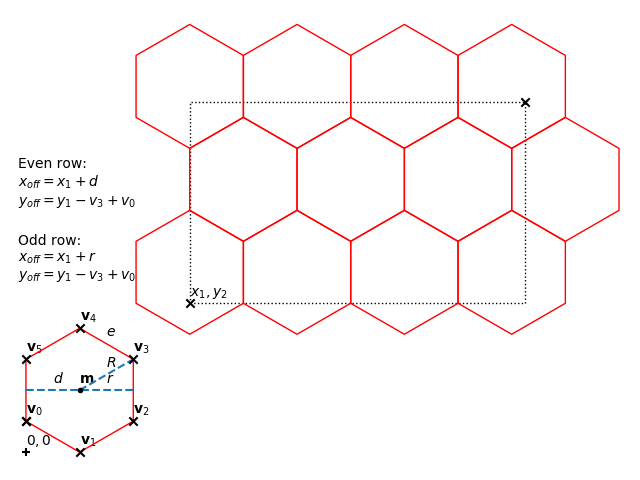
\includegraphics[scale=.66]{img/hexagons}
			\caption[Hexagon tessellation]{\textbf{Hexagon tessellation:} Located at the left bottom corner in red a hexagon defined by its geometric properties the 6 vertex vectors \{$\vec{v_0},...,\vec{v_5}$\} (black crosses), with center vector $\vec{m}$, edge length $e$, $R$ radius of the circumscribing circle, $r$ radius of the inscribed circle and $d$ the short diagonal (diameter of the inscribed circle). Top right black dotted box are the bounds of an area which is tessellated by a hexagon grid in red. Each grid cell is translated from the origin hexagon at its position by computing the $x_{off}$ and $y_{off}$ offset with the presented equations at the left-hand side of the grid. }
			\label{fig:hexagon}
		\end{figure}

		To create a polygon grid of a plane image we must align several hexagons to cover the image. For our tessellation algorithm we use the vertex matrix $\mathbf{H}$ computed by the previously described approach and subsequently translate it to its position within the grid. We expect to receive the bounds matrix $\mathbf{B}$ of the raster image which should be tessellated by hexagons, equation \ref{eq:hexagon_bounds}. Let $x_1$, $y_1$ be the left bottom corner coordinates and $x_2$, $y_2$ the right top corner coordinates of an image. Let $x_{off}(0)$, $y_{off}(0)$ in equation \ref{eq:hexagon_x_off_start} and \ref{eq:hexagon_y_off_start} be the initial coordinates for creating a polygon grid over a plane. Then we can obtain $x_{off}(n+1)$ the $x$ coordinates for even rows by applying equation \ref{eq:hexagon_x_off_even} and $x_{off}(n+1)$ the $x$ coordinates for odd rows by equation \ref{eq:hexagon_x_off_odd}. Where $r$ is the radius of an inscribed circle in a hexagon and can be obtained by dividing $d$ by 2. Then $\mathbf{H}$ can be translated to the vertex matrix $\mathbf{T}$ by applying the dot product of an affine transformation matrix and $\mathbf{H}$, equation \ref{eq:hexagon_translate}.
		\begin{equation}
		\label{eq:hexagon_bounds}
			\mathbf{B} =
				\begin{bmatrix}
				x_1 & x_2 \\
				y_1 & y_2
			\end{bmatrix}
		\end{equation}
		\begin{equation}
		\label{eq:hexagon_x_off_start}
			x_{off}(0)=x_1
		\end{equation}
		\begin{equation}
		\label{eq:hexagon_y_off_start}
			y_{off}(0)=y_1
		\end{equation}
		\begin{equation}
		\label{eq:hexagon_x_off_even}
			x_{off}(n+1)=x_{off}(n)+d
		\end{equation}
		\begin{equation}
		\label{eq:hexagon_x_off_odd}
			x_{off}(n+1)=x_{off}(n)-r+d
		\end{equation}
		\begin{equation}
		\label{eq:hexagon_y_off}
			y_{off}(n+1)=y_{off}(n)-v_{0,2}+v_{3,2}
		\end{equation}
		\begin{equation}
		\label{eq:hexagon_translate}
		\mathbf{T} =
			\begin{bmatrix}
				1 & 0 & x_{off}(n) \\
				0 & 1 & y_{off}(n) \\
				0 & 0 & 1
			\end{bmatrix} \circ \mathbf{H}
		\end{equation}

		Goal: A pie chart within the area of a hexagon, split the hexagon in horizontal pieces which represent a ratio

		How: Compute the y coordinate of the split line from the ratio, the distance between y1 and y2, compute from this the x coordinates
		\begin{equation}
		\label{eq:hexagon_ratio}
			y = \frac{P(y_2-y_1)}{100} + y_1
		\end{equation}
		\begin{equation}
		\label{eq:hexagon_left_intersection}
			f^{-1}(y) =
			\begin{cases} 
				-\frac{y - y_1}{\tan{(\frac{\pi}{6}})} + \frac{x_1 + x_2}{2} & \text{if } y_1 \le y < y_1 + R\sin{(\frac{5\pi}{6})} \\
				x_1 & \text{if } y_1 + R\sin{(\frac{5\pi}{6})} \le y < R(\sin{(\frac{5\pi}{6})} + 1) \\
				\frac{y - y_2}{\tan{(\frac{\pi}{6}})} + \frac{x_1 + x_2}{2} & \text{if } R(\sin{(\frac{5\pi}{6})} + 1) \le y \le y_2
			\end{cases}
		\end{equation}
		\begin{equation}
		\label{eq:hexagon_right_intersection}
			g^{-1}(y) = 
			\begin{cases} 
				\frac{y - y_1}{\tan{(\frac{\pi}{6}})} + \frac{x_1 + x_2}{2} & \text{if } y_1 \le y < y_1 + R\sin{(\frac{5\pi}{6})} \\
				x_2 & \text{if } y_1 + R\sin{(\frac{5\pi}{6})} \le y < R(\sin{(\frac{5\pi}{6})} + 1) \\
				-\frac{y - y_2}{\tan{(\frac{\pi}{6}})} + \frac{x_1 + x_2}{2} & \text{if } R(\sin{(\frac{5\pi}{6})} + 1) \le y \le y_2
			\end{cases}
		\end{equation}
		\begin{equation}
		\label{eq:hexagon_split_line}
			\mathbf{L} =
			\begin{bmatrix}
				f^{-1}(y) & g^{-1}(y) \\
				y & y
			\end{bmatrix}
		\end{equation}

		Goal: All use hexagons with an area of 0.5 degrees i square, aggregated tiles per continent americas, africa, asia

		Treecover: Count tree cover pixels within hexagon in canopy interval (10,100], count total pixels within hexagon, compute pixel area with haversine, divide tree covered area by total area, 5 ratio bins 0.2 0.4 0.6 0.8 1.0 for scaling, store the area for interval, mean canopy density over occupied pixels, use mean canopy density for choropleth map

		Loss: count frequency of pdd recognized as deforestation 

		PDD: count frequencies within a hexagon, compute frequency ratios, segement hexagons by the ratio of pdd driver, order the drivers in decreasing order, most common is first, tried with scaling but not feasible cause few big sized and many small sized, just scale them a bit down cause visual appeal,

		Hexagonal Country-boundaries: Hexagon grid over the continent aggregate cells which cover a country, vastly made by hand